\documentclass[aspectratio=169,12pt]{beamer}
\usepackage[utf8]{inputenc}
\usepackage[T1]{fontenc}
\usepackage{amsmath, amssymb}
\usepackage{booktabs}
\usepackage{colortbl}
\usepackage{hyperref}
\usepackage{makecell}
\usepackage{ragged2e}
\usepackage{tikz}
\usetikzlibrary{arrows.meta, positioning, shapes.geometric, calc, tikzmark, shapes.misc, matrix, patterns, fit, decorations.pathmorphing, shapes.callouts}
\usepackage{tcolorbox}
\usepackage{listings}
\lstset{
    basicstyle=\ttfamily\scriptsize,
    keywordstyle=\color{blue},
    commentstyle=\color{green!50!black},
    stringstyle=\color{red},
    showstringspaces=false,
    frame=single,
    backgroundcolor=\color{gray!10},
    xleftmargin=0.5em,
    xrightmargin=0.5em,
}

\usetheme{Madrid}
\usecolortheme{default}

% Custom colors
\definecolor{mygreen}{RGB}{0,128,0}
\definecolor{myblue}{RGB}{0,0,255}
\definecolor{myred}{RGB}{255,0,0}
\definecolor{thread0}{RGB}{100,149,237}
\definecolor{thread1}{RGB}{255,165,0}

\title{Multi-Threading}
\author{Computer Architecture 2360267}
\date{2025, Lecture \#12}

\begin{document}

\frame{\titlepage}

% Table of Contents
\begin{frame}{Outline}
\tableofcontents
\end{frame}

\section{Parallelism}

% Slide 2: Parallelism
\begin{frame}{Parallelism}
\begin{itemize}
    \item \textbf{Instruction Level Parallelism (ILP)}
    \begin{itemize}
        \item Independent instructions within a program can run in parallel
        \item A given program, with a given input data has a given parallelism
        \item An OOO machine extracts ILP allowing independent instructions to run in parallel
    \end{itemize}
    \item \textbf{Data Level Parallelism (DLP)}
    \begin{itemize}
        \item Same operation executed on multiple data elements
        \item E.g., adding two vectors: same add operation applied to each pair of elements
    \end{itemize}
    \item \textbf{Thread Level Parallelism (TLP)}
    \begin{itemize}
        \item A threaded application: an application written to use multiple threads
        \item Multi-threaded code is hard to write, to debug, and to validate
        \item Different applications running simultaneously
        \item Operating system services running in parallel to applications
    \end{itemize}
\end{itemize}
\end{frame}

\section{Single-Core Multi-Threading}

% Slide 3: Single-Core Multi-Threading
\begin{frame}{Single-Core Multi-Threading}
\begin{itemize}
    \item \textbf{Multi-threading}: a single core executes multiple threads
    \item When one thread is stalled (on a cache miss, branch misprediction, or a long dependency), the other thread gets to use the free resources
    \vspace{0.3cm}
    \item \textbf{Switch-on-event multithreading (SOEMT)}
    \begin{itemize}
        \item A single thread exists in the machine at a given moment
        \item Switch threads on a long latency event, such as last level cache misses
        \item Works well for server applications that have many cache misses
        \item Does not cover for branch mispredictions and single-thread low ILP
    \end{itemize}
    \vspace{0.3cm}
    \item \textbf{Simultaneous multi-threading (SMT)}
    \begin{itemize}
        \item Multiple threads execute on a single core simultaneously
        \item Interleaved in the machine pipeline
        \item When one thread is stalled / slowed down, other thread gets more resources
        \item Makes the most effective use of processor resources
    \end{itemize}
\end{itemize}
\end{frame}

% Slide 4: Core Resources Utilization
\begin{frame}{Core Resources Utilization}
\begin{itemize}
    \item \textbf{The IPC of a program is limited due to:}
    \begin{itemize}
        \item Instruction dependencies (ILP -- Instruction Level Parallelism)
        \item Cache misses
        \item Branch misprediction
        \item Memory bound vs.\ compute bound workloads
    \end{itemize}
    \vspace{0.3cm}
    \item \textbf{Server apps are typically memory bound, with low IPC}
    \begin{itemize}
        \item Actual average IPC for a 4-wide machine is $<2$
        \item Utilization $< 50\%$
        \item Even taking into account that 10\%-20\% more instructions are fetched and executed than retired due to speculative execution
    \end{itemize}
    \vspace{0.3cm}
    \item \textbf{Increasing single thread performance becomes harder}
    \begin{itemize}
        \item Less power efficient, less area efficient
    \end{itemize}
\end{itemize}
\end{frame}

\section{Simultaneous Multi-Threading (SMT)}

% Slide 5: Simultaneous multi-threading (SMT)
\begin{frame}{Simultaneous Multi-Threading (SMT)}
\begin{columns}[T]
\column{0.55\textwidth}
\begin{itemize}
    \item \textbf{Two logical processors within one physical core}
    \begin{itemize}
        \item Sharing most execution/cache resources using SMT
        \item Look like two processors to the SW (OS and apps)
    \end{itemize}
    \item \textbf{Each logical processor executes a software thread}
    \begin{itemize}
        \item Threads execute simultaneously on one physical core
    \end{itemize}
    \item \textbf{Each logical processor maintains its own arch.\ state}
    \begin{itemize}
        \item Complete set of architectural registers
        \item General-purpose registers
        \item Instruction pointers
        \item Control registers and Machine state registers
        \item Debug registers
    \end{itemize}
    \item \textbf{Each logical processor has its own interrupt controller}
    \begin{itemize}
        \item Handles interrupts sent to the specific logical processor
    \end{itemize}
\end{itemize}

\column{0.4\textwidth}
\centering
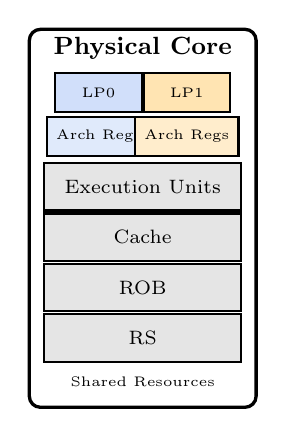
\begin{tikzpicture}[scale=0.8,
    box/.style={draw, thick, minimum width=2.5cm, minimum height=0.6cm, font=\scriptsize},
    smallbox/.style={draw, thick, minimum width=1.1cm, minimum height=0.5cm, font=\tiny}
]
    % Physical Core outline
    \draw[very thick, rounded corners] (-1.8,-3.5) rectangle (1.8,2.5);
    \node[font=\small\bfseries] at (0,2.2) {Physical Core};

    % Two logical processors
    \node[smallbox, fill=thread0!30] (lp0) at (-0.7,1.5) {LP0};
    \node[smallbox, fill=thread1!30] (lp1) at (0.7,1.5) {LP1};

    % Arch state
    \node[smallbox, fill=thread0!20] at (-0.7,0.8) {Arch Regs};
    \node[smallbox, fill=thread1!20] at (0.7,0.8) {Arch Regs};

    % Shared resources
    \node[box, fill=gray!20] (exec) at (0,0) {Execution Units};
    \node[box, fill=gray!20] (cache) at (0,-0.8) {Cache};
    \node[box, fill=gray!20] (rob) at (0,-1.6) {ROB};
    \node[box, fill=gray!20] (rs) at (0,-2.4) {RS};

    % Label
    \node[font=\tiny, align=center] at (0,-3.1) {Shared Resources};
\end{tikzpicture}
\end{columns}
\end{frame}

% Slide 6: SMT Physical Resource Sharing Schemes
\begin{frame}{SMT Physical Resource Sharing Schemes}
\begin{columns}[T]
\column{0.74\textwidth}
\vspace{-0.4cm}
\begin{itemize}
    \item \textbf{Replicated Resources}: each thread has its own resource (e.g., renaming tables)
    \item \textbf{Partitioned Resources}: resource is partitioned in MT mode, combined in ST mode (e.g., ROB)
    \item \textbf{Competitively-shared}: both threads compete for the entire resource (e.g., RS entries -- may have minimum guarantee per thread)
    \item \textbf{Thread-unaware}: both threads use the resource (e.g., execution units)
\end{itemize}

\vspace{-0.1cm}
\begin{alertblock}{Resource Sharing May Cause Performance Issues}
E.g., \textbf{cache thrashing}: the workload run by each thread fits into the cache, but both workloads together don't fit into the cache $\Rightarrow$ high miss rate
\end{alertblock}

\column{0.24\textwidth}
\centering
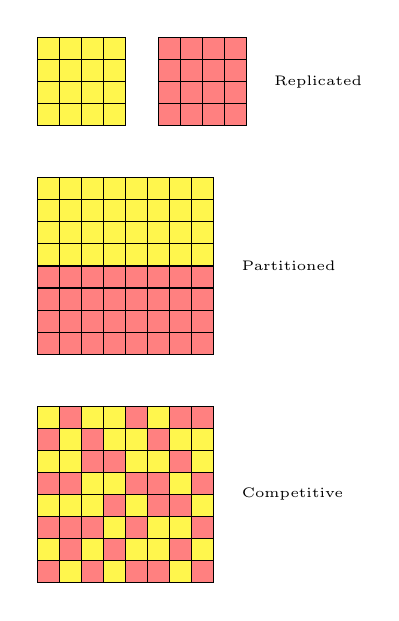
\begin{tikzpicture}[
    cell/.style={minimum width=0.28cm, minimum height=0.28cm, draw, inner sep=0pt},
    t0/.style={fill=yellow!70},
    t1/.style={fill=red!50},
    shared/.style={fill=blue!20},
    matrixstyle/.style={matrix of nodes, ampersand replacement=\&, nodes={cell}, row sep=-\pgflinewidth, column sep=-\pgflinewidth}
]
% Replicated - two separate matrices
\matrix[matrixstyle, nodes={cell, t0}] (rep0) at (0,0) {
 ~ \& ~ \& ~ \& ~ \\
 ~ \& ~ \& ~ \& ~ \\
 ~ \& ~ \& ~ \& ~ \\
 ~ \& ~ \& ~ \& ~ \\
};
\matrix[matrixstyle, nodes={cell, t1}, right=0.15cm of rep0] (rep1) {
 ~ \& ~ \& ~ \& ~ \\
 ~ \& ~ \& ~ \& ~ \\
 ~ \& ~ \& ~ \& ~ \\
 ~ \& ~ \& ~ \& ~ \\
};
\node[font=\tiny, right=0.1cm of rep1] {Replicated};

% Partitioned - one matrix, top half yellow, bottom half red
\matrix[matrixstyle, below=0.4cm of rep0.south west, anchor=north west] (part) {
 |[t0]| ~ \& |[t0]| ~ \& |[t0]| ~ \& |[t0]| ~ \& |[t0]| ~ \& |[t0]| ~ \& |[t0]| ~ \& |[t0]| ~ \\
 |[t0]| ~ \& |[t0]| ~ \& |[t0]| ~ \& |[t0]| ~ \& |[t0]| ~ \& |[t0]| ~ \& |[t0]| ~ \& |[t0]| ~ \\
 |[t0]| ~ \& |[t0]| ~ \& |[t0]| ~ \& |[t0]| ~ \& |[t0]| ~ \& |[t0]| ~ \& |[t0]| ~ \& |[t0]| ~ \\
 |[t0]| ~ \& |[t0]| ~ \& |[t0]| ~ \& |[t0]| ~ \& |[t0]| ~ \& |[t0]| ~ \& |[t0]| ~ \& |[t0]| ~ \\
 |[t1]| ~ \& |[t1]| ~ \& |[t1]| ~ \& |[t1]| ~ \& |[t1]| ~ \& |[t1]| ~ \& |[t1]| ~ \& |[t1]| ~ \\
 |[t1]| ~ \& |[t1]| ~ \& |[t1]| ~ \& |[t1]| ~ \& |[t1]| ~ \& |[t1]| ~ \& |[t1]| ~ \& |[t1]| ~ \\
 |[t1]| ~ \& |[t1]| ~ \& |[t1]| ~ \& |[t1]| ~ \& |[t1]| ~ \& |[t1]| ~ \& |[t1]| ~ \& |[t1]| ~ \\
 |[t1]| ~ \& |[t1]| ~ \& |[t1]| ~ \& |[t1]| ~ \& |[t1]| ~ \& |[t1]| ~ \& |[t1]| ~ \& |[t1]| ~ \\
};
\node[font=\tiny, right=0.1cm of part.east] {Partitioned};

% Competitive - mixed pattern
\matrix[matrixstyle, below=0.4cm of part.south west, anchor=north west] (comp) {
 |[t0]| ~ \& |[t1]| ~ \& |[t0]| ~ \& |[t0]| ~ \& |[t1]| ~ \& |[t0]| ~ \& |[t1]| ~ \& |[t1]| ~ \\
 |[t1]| ~ \& |[t0]| ~ \& |[t1]| ~ \& |[t0]| ~ \& |[t0]| ~ \& |[t1]| ~ \& |[t0]| ~ \& |[t0]| ~ \\
 |[t0]| ~ \& |[t0]| ~ \& |[t1]| ~ \& |[t1]| ~ \& |[t0]| ~ \& |[t0]| ~ \& |[t1]| ~ \& |[t0]| ~ \\
 |[t1]| ~ \& |[t1]| ~ \& |[t0]| ~ \& |[t0]| ~ \& |[t1]| ~ \& |[t1]| ~ \& |[t0]| ~ \& |[t1]| ~ \\
 |[t0]| ~ \& |[t0]| ~ \& |[t0]| ~ \& |[t1]| ~ \& |[t0]| ~ \& |[t1]| ~ \& |[t1]| ~ \& |[t0]| ~ \\
 |[t1]| ~ \& |[t1]| ~ \& |[t1]| ~ \& |[t0]| ~ \& |[t1]| ~ \& |[t0]| ~ \& |[t0]| ~ \& |[t1]| ~ \\
 |[t0]| ~ \& |[t1]| ~ \& |[t0]| ~ \& |[t1]| ~ \& |[t0]| ~ \& |[t0]| ~ \& |[t1]| ~ \& |[t0]| ~ \\
 |[t1]| ~ \& |[t0]| ~ \& |[t1]| ~ \& |[t0]| ~ \& |[t1]| ~ \& |[t1]| ~ \& |[t0]| ~ \& |[t1]| ~ \\
};
\node[font=\tiny, right=0.1cm of comp.east] {Competitive};
\end{tikzpicture}
\end{columns}
\end{frame}

% Slide 7: SMT Resource Sharing Table
\begin{frame}{SMT Resource Sharing}
\centering
\small
\begin{tabular}{l|l|l|l}
\toprule
\textbf{Sharing Type} & \textbf{Frontend} & \textbf{OOO/EXE} & \textbf{Memory} \\
\midrule
\textbf{Replicated} & Instruction Pointer & \makecell[l]{Arch.\ registers\\Renaming table} & Interrupt controller \\
\midrule
\textbf{Partitioned} & Instruction TLB & ROB & \makecell[l]{Load buffers\\Store buffers} \\
\midrule
\textbf{Competitive} & Branch prediction & RS & \makecell[l]{Data TLB\\2nd Level TLB} \\
\midrule
\textbf{Thread-unaware} & I\$, decoders & Execution units & D\$ \\
\bottomrule
\end{tabular}
\end{frame}

% Slide 8: SMT: A High-level View of the Pipeline
\begin{frame}{SMT: A High-level View of the Pipeline}
\begin{itemize}
    \item Each pipe-stage is occupied by one of the threads
\end{itemize}

\vspace{0.1cm}
\centering
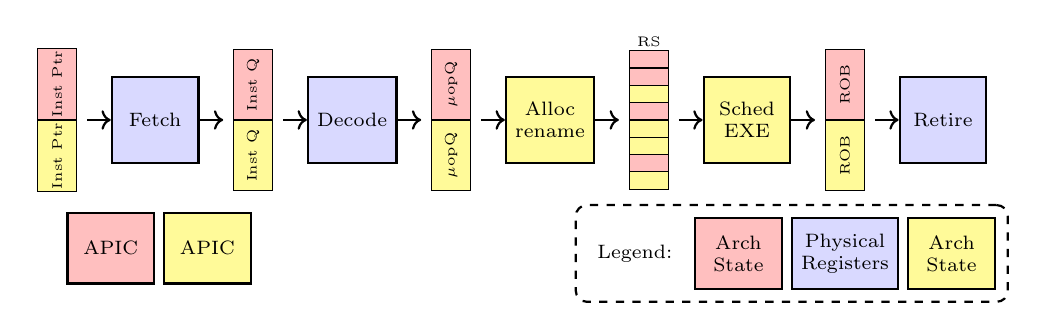
\begin{tikzpicture}[
    % Styles
    pipestage/.style={draw, thick, minimum width=1.1cm, minimum height=1.1cm, font=\scriptsize, fill=blue!15, align=center},
    % For rotated text: min width becomes visual height, min height becomes visual width
    latchcell/.style={draw, minimum width=0.9cm, minimum height=0.5cm, font=\tiny, inner sep=1pt},
    latch t0/.style={fill=red!25},
    latch t1/.style={fill=yellow!40},
    latchmatrix/.style={matrix of nodes, ampersand replacement=\&, row sep=-\pgflinewidth, column sep=0pt,
                        nodes={latchcell}},
    % RS: 8 cells @ 0.275cm each = 2.2cm total height
    rscell/.style={draw, minimum width=0.5cm, minimum height=0.22cm, inner sep=0pt},
    rs t0/.style={fill=red!25},
    rs t1/.style={fill=yellow!40},
    rsmatrix/.style={matrix of nodes, ampersand replacement=\&, row sep=-\pgflinewidth, column sep=0pt,
                     nodes={rscell}},
    bottombox/.style={draw, thick, minimum width=1.1cm, minimum height=0.9cm, font=\scriptsize, align=center},
    node distance=0.15cm
]
    % Inst Ptr latches (replicated, stacked vertically)
    \matrix[latchmatrix] (instptr) {
        |[latch t0, rotate=90]| Inst Ptr \\
        |[latch t1, rotate=90]| Inst Ptr \\
    };

    % Fetch stage
    \node[pipestage, right=0.3cm of instptr] (fetch) {Fetch};

    % Inst Q latches (replicated, stacked vertically)
    \matrix[latchmatrix, right=0.3cm of fetch] (instq) {
        |[latch t0, rotate=90]| Inst Q \\
        |[latch t1, rotate=90]| Inst Q \\
    };

    % Decode stage
    \node[pipestage, right=0.3cm of instq] (decode) {Decode};

    % uopQ latches (replicated, stacked vertically)
    \matrix[latchmatrix, right=0.3cm of decode] (uopq) {
        |[latch t0, rotate=90]| $\mu$opQ \\
        |[latch t1, rotate=90]| $\mu$opQ \\
    };

    % Alloc/Rename stage
    \node[pipestage, right=0.3cm of uopq, fill=yellow!40] (alloc) {Alloc\\rename};

    % RS (shared with mixed thread entries, single column)
    \matrix[rsmatrix, right=0.3cm of alloc] (rs) {
        |[rs t0]| ~ \\
        |[rs t0]| ~ \\
        |[rs t1]| ~ \\
        |[rs t0]| ~ \\
        |[rs t1]| ~ \\
        |[rs t1]| ~ \\
        |[rs t0]| ~ \\
        |[rs t1]| ~ \\
    };
    \node[font=\tiny, above=-2mm of rs] {RS};

    % Sched/EXE stage
    \node[pipestage, right=0.3cm of rs, fill=yellow!40] (sched) {Sched\\EXE};

    % ROB latches (replicated, stacked vertically)
    \matrix[latchmatrix, right=0.3cm of sched] (rob) {
        |[latch t0, rotate=90]| ROB \\
        |[latch t1, rotate=90]| ROB \\
    };

    % Retire stage
    \node[pipestage, right=0.3cm of rob] (retire) {Retire};

    % Arrows connecting stages
    \draw[->, thick] (instptr.east) -- (fetch.west);
    \draw[->, thick] (fetch.east) -- (instq.west);
    \draw[->, thick] (instq.east) -- (decode.west);
    \draw[->, thick] (decode.east) -- (uopq.west);
    \draw[->, thick] (uopq.east) -- (alloc.west);
    \draw[->, thick] (alloc.east) -- (rs.west);
    \draw[->, thick] (rs.east) -- (sched.west);
    \draw[->, thick] (sched.east) -- (rob.west);
    \draw[->, thick] (rob.east) -- (retire.west);

    % Bottom row - APIC boxes
    \node[bottombox, fill=red!25, below=0.6cm of fetch.south west, anchor=north] (apic0) {APIC};
    \node[bottombox, fill=yellow!40, right=0.1cm of apic0] (apic1) {APIC};

    % Bottom row - Register boxes with legend (positioned relative to ROB)
    \node[bottombox, fill=blue!15, below=0.2cm of rob.south, anchor=north] (physreg) {Physical\\Registers};
    \node[bottombox, fill=red!25, left=0.1cm of physreg] (archstate0) {Arch\\State};
    \node[bottombox, fill=yellow!40, right=0.1cm of physreg] (archstate1) {Arch\\State};
    \node[font=\scriptsize, left=0.15cm of archstate0.west, anchor=east] (legendlabel) {Legend:};

    % Dashed border around legend
    \node[draw, dashed, thick, rounded corners, inner sep=0.15cm, fit=(legendlabel)(archstate0)(physreg)(archstate1)] {};
\end{tikzpicture}

\vspace{0.3cm}
\begin{columns}[T]
\column{0.5\textwidth}
\begin{itemize}\small
    \item Per pipe-stage \textbf{thread bit} indicates which thread is currently occupying the pipe-stage
    \item In case of a flush (e.g., branch misprediction), flush only the specific thread
\end{itemize}

\column{0.5\textwidth}
\begin{itemize}\small
    \item When one thread is stalled, the other thread can continue to make progress
    \item \textbf{Pipe-stages}: either guaranteed not to stall, or flushed if preventing other thread from progress
    \item \textbf{Buffers}: partitioned / replicated / shared with guaranteed entries
\end{itemize}
\end{columns}
\end{frame}

% Slide 9: SMT Thread Select Points
\begin{frame}{SMT Thread Select Points}
\centering
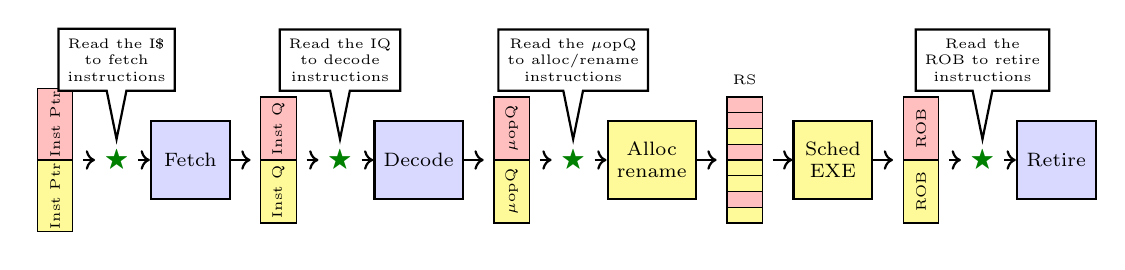
\begin{tikzpicture}[
    % Styles
    pipestage/.style={draw, thick, minimum width=1.0cm, minimum height=1.0cm, font=\scriptsize, fill=blue!15, align=center},
    latchcell/.style={draw, minimum width=0.8cm, minimum height=0.45cm, font=\tiny, inner sep=1pt},
    latch t0/.style={fill=red!25},
    latch t1/.style={fill=yellow!40},
    latchmatrix/.style={matrix of nodes, ampersand replacement=\&, row sep=-\pgflinewidth, column sep=0pt, nodes={latchcell}},
    rscell/.style={draw, minimum width=0.45cm, minimum height=0.2cm, inner sep=0pt},
    rs t0/.style={fill=red!25},
    rs t1/.style={fill=yellow!40},
    rsmatrix/.style={matrix of nodes, ampersand replacement=\&, row sep=-\pgflinewidth, column sep=0pt, nodes={rscell}},
    star/.style={font=\small, text=green!50!black},
    mycallout/.style={rectangle callout, draw, thick, fill=white, font=\tiny, align=center},
    node distance=0.12cm
]
    % Inst Ptr latches (replicated, stacked vertically)
    \matrix[latchmatrix] (instptr) {
        |[latch t0, rotate=90]| Inst Ptr \\
        |[latch t1, rotate=90]| Inst Ptr \\
    };

    % Star 1 - between Inst Ptr and Fetch
    \node[star, right=0.15cm of instptr] (star1) {$\bigstar$};

    % Fetch stage
    \node[pipestage, right=0.15cm of star1] (fetch) {Fetch};

    % Inst Q latches (replicated, stacked vertically)
    \matrix[latchmatrix, right=0.25cm of fetch] (instq) {
        |[latch t0, rotate=90]| Inst Q \\
        |[latch t1, rotate=90]| Inst Q \\
    };

    % Star 2 - between Inst Q and Decode
    \node[star, right=0.15cm of instq] (star2) {$\bigstar$};

    % Decode stage
    \node[pipestage, right=0.15cm of star2] (decode) {Decode};

    % uopQ latches (replicated, stacked vertically)
    \matrix[latchmatrix, right=0.25cm of decode] (uopq) {
        |[latch t0, rotate=90]| $\mu$opQ \\
        |[latch t1, rotate=90]| $\mu$opQ \\
    };

    % Star 3 - between uopQ and Alloc
    \node[star, right=0.15cm of uopq] (star3) {$\bigstar$};

    % Alloc/Rename stage
    \node[pipestage, right=0.15cm of star3, fill=yellow!40] (alloc) {Alloc\\rename};

    % RS (shared with mixed thread entries, single column)
    \matrix[rsmatrix, right=0.25cm of alloc] (rs) {
        |[rs t0]| ~ \\
        |[rs t0]| ~ \\
        |[rs t1]| ~ \\
        |[rs t0]| ~ \\
        |[rs t1]| ~ \\
        |[rs t1]| ~ \\
        |[rs t0]| ~ \\
        |[rs t1]| ~ \\
    };
    \node[font=\tiny, above=-1mm of rs] {RS};

    % Sched/EXE stage
    \node[pipestage, right=0.25cm of rs, fill=yellow!40] (sched) {Sched\\EXE};

    % ROB latches (replicated, stacked vertically)
    \matrix[latchmatrix, right=0.25cm of sched] (rob) {
        |[latch t0, rotate=90]| ROB \\
        |[latch t1, rotate=90]| ROB \\
    };

    % Star 4 - between ROB and Retire
    \node[star, right=0.15cm of rob] (star4) {$\bigstar$};

    % Retire stage
    \node[pipestage, right=0.15cm of star4] (retire) {Retire};

    % Arrows connecting stages
    \draw[->, thick] (instptr.east) -- (star1.west);
    \draw[->, thick] (star1.east) -- (fetch.west);
    \draw[->, thick] (fetch.east) -- (instq.west);
    \draw[->, thick] (instq.east) -- (star2.west);
    \draw[->, thick] (star2.east) -- (decode.west);
    \draw[->, thick] (decode.east) -- (uopq.west);
    \draw[->, thick] (uopq.east) -- (star3.west);
    \draw[->, thick] (star3.east) -- (alloc.west);
    \draw[->, thick] (alloc.east) -- (rs.west);
    \draw[->, thick] (rs.east) -- (sched.west);
    \draw[->, thick] (sched.east) -- (rob.west);
    \draw[->, thick] (rob.east) -- (star4.west);
    \draw[->, thick] (star4.east) -- (retire.west);

    % Callout bubbles
    \node[mycallout, callout absolute pointer={(star1.north)}, above=0.6cm of star1] (c1) {Read the I\$\\to fetch\\instructions};
    \node[mycallout, callout absolute pointer={(star2.north)}, above=0.6cm of star2] (c2) {Read the IQ\\to decode\\instructions};
    \node[mycallout, callout absolute pointer={(star3.north)}, above=0.6cm of star3] (c3) {Read the $\mu$opQ\\to alloc/rename\\instructions};
    \node[mycallout, callout absolute pointer={(star4.north)}, above=0.6cm of star4] (c4) {Read the\\ROB to retire\\instructions};
\end{tikzpicture}

\vspace{0.3cm}
\begin{columns}[T]
\column{0.5\textwidth}
\begin{itemize}\small
    \item \textbf{Pipeline arbitration points} ($\bigstar$) select the thread that gets to use a resource in a given cycle
    \begin{itemize}
        \item ``ping-pong'' between the threads on a cycle-by-cycle basis
        \item If one thread is stalled $\Rightarrow$ give its turn to the other thread
    \end{itemize}
\end{itemize}

\column{0.5\textwidth}
\begin{itemize}\small
    \item \textbf{The RS is not a thread arbitration point}
    \begin{itemize}
        \item Dispatches $\mu$ops to EUs based on readiness and age
        \item Regardless of which thread they belong to
    \end{itemize}
\end{itemize}
\end{columns}
\end{frame}

% Slide 10: Single-task And Multi-task Modes
\begin{frame}{Single-task And Multi-task Modes}
\begin{columns}[T]
\column{0.45\textwidth}
\begin{itemize}
    \item \textbf{MT-mode (Multi-task mode)}
    \begin{itemize}
        \item Two active threads, resources partitioned
    \end{itemize}
    \vspace{0.2cm}
    \item \textbf{ST-mode (Single-task mode)}
    \begin{itemize}
        \item ST0 / ST1 -- only thread 0 / 1 is active
        \item Partitioned resources re-combined for single thread
    \end{itemize}
    \vspace{0.2cm}
    \item \textbf{Low Power mode}
    \begin{itemize}
        \item Both threads halted
    \end{itemize}
\end{itemize}

\column{0.55\textwidth}
\centering
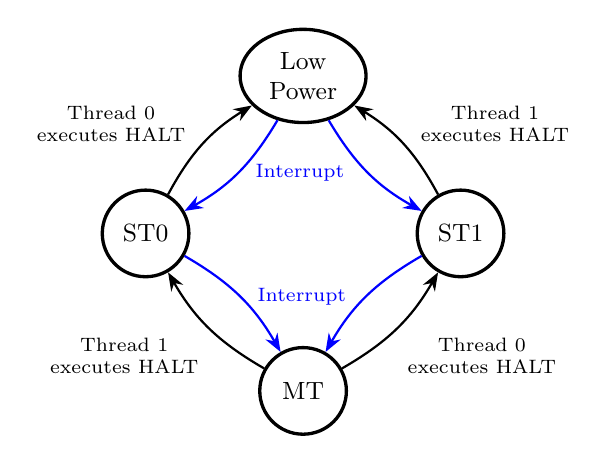
\begin{tikzpicture}[
    state/.style={draw, very thick, circle, minimum size=1.1cm, font=\small},
    ellstate/.style={draw, very thick, ellipse, minimum width=1.6cm, minimum height=1.1cm, font=\small, align=center},
    haltarrow/.style={->, thick, >=Stealth},
    intarrow/.style={->, thick, >=Stealth, blue},
    labelstyle/.style={font=\scriptsize, align=center}
]
    % States in diamond pattern
    \node[ellstate] (lp) at (0,2) {Low\\Power};
    \node[state] (st0) at (-2,0) {ST0};
    \node[state] (st1) at (2,0) {ST1};
    \node[state] (mt) at (0,-2) {MT};

    % Black arrows - Thread executes HALT
    \draw[haltarrow, bend left=15] (st0) to node[labelstyle, above left, pos=0.4] {Thread 0\\executes HALT} (lp);
    \draw[haltarrow, bend right=15] (st1) to node[labelstyle, above right, pos=0.4] {Thread 1\\executes HALT} (lp);
    \draw[haltarrow, bend left=15] (mt) to node[labelstyle, below left, pos=0.5] {Thread 1\\executes HALT} (st0);
    \draw[haltarrow, bend right=15] (mt) to node[labelstyle, below right, pos=0.5] {Thread 0\\executes HALT} (st1);

    % Blue arrows - Interrupt (labeled on outer side of curve)
    \draw[intarrow, bend left=15] (lp) to node[labelstyle, right, blue, pos=0.5] {~Interrupt} (st0);
    \draw[intarrow, bend right=15] (lp) to node[labelstyle, left, blue, pos=0.5] {} (st1);
    \draw[intarrow, bend left=15] (st0) to node[labelstyle, right, blue, pos=0.5] {~Interrupt} (mt);
    \draw[intarrow, bend right=15] (st1) to node[labelstyle, right, blue, pos=0.5] {} (mt);
\end{tikzpicture}
\end{columns}
\end{frame}

\section{Thread Optimization}

% Slide 11: OS Thread Optimization - HALT
\begin{frame}[fragile]{OS Optimization: Use HALT for Idle Processors}
\begin{itemize}
    \item When a logical processor has no work, OS should execute \texttt{HLT}
    \item Allows transition to ST0/ST1 mode $\rightarrow$ sibling thread gets all resources
\end{itemize}

\vspace{0.2cm}
\begin{columns}[T]
\column{0.48\textwidth}
\textbf{Bad: Busy-wait idle loop}
\begin{lstlisting}[language=C]
void os_idle_loop() {
    while (!work_available) {
        // Spin checking for work
        // Wastes resources!
    }
}
\end{lstlisting}

\column{0.48\textwidth}
\textbf{Good: Use HLT}
\begin{lstlisting}[language=C]
void os_idle_loop() {
    while (!work_available) {
        __halt();
        // Wakes on interrupt
    }
}
\end{lstlisting}
\end{columns}

\vspace{0.3cm}
\begin{itemize}
    \item \texttt{HLT}: stops execution until interrupt arrives
    \begin{itemize}
        \item Enters low power mode, frees execution resources for sibling thread
        \item Without HLT, idle loop consumes significant resources from active thread
    \end{itemize}
\end{itemize}
\end{frame}

% Slide 12: Thread Optimization - Scheduling
\begin{frame}[fragile]{Thread Optimization: Scheduling}
\textbf{On a multi-processor system with SMT:}
\begin{itemize}
    \item OS views logical processors similar to physical processors
    \item But should prefer scheduling on different \textit{physical} cores first
    \item Only use sibling threads (same physical core) when all cores are busy
\end{itemize}

\vspace{0.0cm}
\begin{lstlisting}[language=C, morekeywords={thread_t,cpu_t}]
void schedule_thread(thread_t *thread) {
    // First: try to find an idle physical core
    for (cpu_t *cpu : all_physical_cores) {
        if (cpu->thread0_idle && cpu->thread1_idle) {
            assign(thread, cpu->thread0);  return;
        }
    }
    // Second: use sibling thread on busy core
    for (cpu_t *cpu : all_physical_cores) {
        if (cpu->thread0_idle || cpu->thread1_idle) {
            assign(thread, get_idle_thread(cpu)); return;
        }
    }
    enqueue(thread);  // All CPUs busy, wait in queue
}
\end{lstlisting}
\end{frame}

% Slide 13: User-level Thread Optimization
\begin{frame}[fragile]{User-level Optimization: PAUSE and Affinity}
\begin{columns}[T]
\column{0.48\textwidth}
\textbf{Use PAUSE in spin-wait loops:}
\begin{lstlisting}[language=C]
void spin_lock(int *lock) {
    while (*lock != 0) {
        __pause();
    }
}
\end{lstlisting}
\begin{itemize}\small
    \item Hints CPU: in spin-wait loop
    \item Saves power, avoids memory order violation penalty
    \item Reduces resource contention with sibling thread
\end{itemize}

\column{0.48\textwidth}
\textbf{Set CPU affinity:}
\begin{lstlisting}[language=C]
// Linux: pin thread to CPU 0
cpu_set_t cpuset;
CPU_ZERO(&cpuset);
CPU_SET(0, &cpuset);
pthread_setaffinity_np(
    thread, sizeof(cpuset),
    &cpuset);
\end{lstlisting}
\begin{itemize}\small
    \item User can control which logical CPUs a thread runs on
    \item Avoid sibling threads for cache-sensitive workloads
    \item Or co-locate cooperating threads on same core
\end{itemize}
\end{columns}
\end{frame}

\end{document}
